\documentclass[11pt]{article}

\usepackage[utf8]{inputenc}
\usepackage[T1]{fontenc}
\usepackage[spanish]{babel}

\usepackage{longtable}
\usepackage{amssymb}
\usepackage{amsbsy}
\usepackage{amsmath}
\usepackage{latexsym}%,pstricks,color,epic,eepic}
\usepackage{multicol}
\usepackage{booktabs}
\usepackage{wrapfig}
\usepackage{tabularx}
\usepackage[rightcaption]{sidecap}
\usepackage{csvsimple-l3}
\usepackage{geometry}
\usepackage{graphicx}
\usepackage{pgfplotstable,filecontents}
\pgfplotsset{compat=1.9}% supress warning
\usepackage{eso-pic}
\usepackage{lipsum}
\usepackage{fancyhdr}
\usepackage{float}
%\usepackage[firstpage]{draftwatermark
%\usepackage[doublespace]{setspace}  

\usepackage{draftwatermark}
% Use the following to make modification
%\SetWatermarkAngle{45}
%\SetWatermarkLightness{0.01}
%\SetWatermarkFontSize{3.0cm}
%\SetWatermarkScale{1.0}
\SetWatermarkText{FING, UACH}%\includegraphics{Logo_UACH.png} }

%\usepackage{background}
%\backgroundsetup{contents={\includegraphics[scale=0.4]{Logo_UACH.png}}}
\decimalpoint

%\hoffset = -50pt
%\voffset = -50pt
%\textwidth = 500pt
%\textheight = 615pt

%\texttt{\AddToShipoutPictureBG*
%  {%
%    \put(\LenToUnit{.1\paperwidth}, \LenToUnit{.85\paperheight})
%      {\includegraphics[scale=0.2]{Logo_UACH}}%
%  }
%}
\parskip 1em

\def\IR{{\rm I\!R}}  %for real numbers
\def\IN{{\rm I\!N}}  %for integer numbers
\def\IC{{\rm C}\llap{\vrule height7.1pt width1pt
     depth-.4pt\phantom t}} %for complex numbers \def\covD{{\rmI\!D}}
\def\IQ{{\rm Q}\llap{\vrule height7.7pt width1pt
     depth-.4pt\phantom t}} %for complex numbers \def\covD{{\rmI\!D}}

%   Si pones en tus definiciones las siguientes instrucciones:

\font\cmss=cmss10
\font\cmsss=cmss10 at 7pt

\def\IZ{\relax\ifmmode\mathchoice
{\hbox{\cmss Z\kern-.4em Z}}{\hbox{\cmss Z\kern-.4em Z}}
{\lower.9pt\hbox{\cmsss Z\kern-.4em Z}}
{\lower1.2pt\hbox{\cmsss Z\kern-.4em Z}}\else{\cmss Z\kern-.4em Z}\fi}

%   podr'as usar  $ \IZ $  para denotar los enteros.


%---------------*******************************------------------------


% Definition of title page:
\title{\textsf{
    Reporte Patrones de resiliencia\\
Laboratorio de Sistemas Complejos}}
\author{Cristian Yael Rubi Loera}
%\pagestyle{headings}
\date{octubre 2024}
%{10 de octubre de 2006}

% Definition of \maketitle
\pagenumbering{Roman}

\begin{document}

 \begin{minipage}[t]{\textwidth}
   \centering
   \raisebox{-\baselineskip}{\rule{\textwidth}{1px}}
   \rule{\textwidth}{1px}
   \vspace{0.2cm}
   \maketitle
   \rule{\textwidth}{2px}
 \end{minipage}
 
\newpage

\pagenumbering{arabic}
\setcounter{page}{2}

\section{Replicación de resultados de en redes mutualistas}


Con base en la información suplementaria del artículo~\cite{gao2016universal}.
Como matriz de interacción para la simulación se tomó la siguiente matriz de $26 \times 10$ de un ecosistema de peces y anémonas (por simplicidad, se refiere estas interacciones como polinizadores y plantas respectivamente, estos roles se mantienen para los demás ecosistemas con redes mutualistas):

\begin{equation*}
M_{mn}=\begin{vmatrix}
1&1&1&1&1&1&1&1&1&1\\
1&1&1&1&1&1&1&0&0&0\\
1&1&1&1&1&0&1&1&0&0\\
0&0&1&1&1&0&1&0&0&0\\
1&1&1&1&1&1&0&0&0&0\\
1&1&0&1&1&0&0&0&0&0\\
1&0&1&0&0&1&0&1&0&0\\
0&1&0&1&1&0&0&0&0&0\\
1&1&1&0&0&1&0&0&0&0\\
0&0&1&1&0&1&0&0&0&0\\
1&0&1&0&0&1&0&0&0&0\\
1&0&1&1&0&0&0&0&0&0\\
1&0&0&0&0&0&1&1&0&0\\
1&1&0&0&0&0&1&0&0&0\\
0&1&0&0&0&1&0&0&0&0\\
1&0&0&1&0&0&0&0&0&0\\
0&0&1&1&0&0&0&0&0&0\\
1&1&0&0&0&0&0&0&0&0\\
0&1&0&0&0&0&0&0&0&0\\
0&0&0&1&0&0&0&0&0&0\\
1&0&0&0&0&0&0&0&0&0\\
0&0&0&1&0&0&0&0&0&0\\
0&1&0&0&0&0&0&0&0&0\\
0&0&1&0&0&0&0&0&0&0\\
0&0&0&0&0&0&1&0&0&0\\
0&1&0&0&0&0&0&0&0&0\\
\end{vmatrix}
\end{equation*}



Partiendo de una matriz de interacción $M_{mn}$ donde $n$ consiste en las plantas y $m$ en los polinizadores, se requiere crear una matriz $A$ dada por: $
A_{ij}=\sum^m_{k=1}\frac{M_{ik}M_{jk}}{\sum^n_{s=1}M_{sk}}
$ para la siguiente ecuación. Puesto que nos interesa modelar la resiliencia de las plantas utilizamos la matriz transpuesta de $M_{mn}^T$ siendo ahora la matriz que utilizaremos la matriz $M_{nm}$.

Ahora podemos resolver la ecuación siguiente, cuya simulación numérica fue realizada usando Runge-Kutta de cuarto orden~\cite{numerical2002recipes}:

\begin{equation}
\label{ec:Diferencial}
\frac{dx_i}{dt} = B_{i}+x_{i}\left( 1-\frac{x_{i}}{K_{i}}\right ) \left(\frac{x_{i}}{C_{i}}-1\right)+\sum^N_{j=1}A_{ij}\frac{x_{i}x_{j}}{D_{i}+E_{i}x_{i}+H_{j}x_{j}}
\end{equation}


Donde para todos los parámetros en la ecuación~\eqref{ec:Diferencial} se usan los siguientes valores constantes:
\begin{eqnarray*}
B_{i}&=&B=0.1,\\
C_{i}&=&C=1,\\
K_{i}&=&K=5,\\ 
D_{i}&=&D=5,\\
E_{i}&=&E=0.9,\\
H_{j}&=&H=0.1\ .
\end{eqnarray*}

En el articulo se utilizan dos estados iniciales $x_{i}(0)=10^{-3}$ y $x_{i}(0)=6.0$, llamados estado inicial bajo($x^{L}$) y estado inicial alto($x^{H}$) .En la figura~\ref{fig-sol-all} se puede observar como las 10 trayectorias simuladas crecen hasta llegar a un punto estable, en este caso usando el estado inicial bajo.

\begin{figure}[H]
\label{fig-sol-all}
\includegraphics[width=10cm, height=10cm]{output_plot_all.png}
\caption{En esta imagen se puede apreciar el crecimiento de las poblaciones en cada iteración de los $n$ polinizadores en la red, de acuerdo con la ecuación diferencial. No se graficó más allá de la iteración 700, ya que a partir de ese punto las poblaciones se estabilizan.}
\end{figure}

Llegado a estos resultados se graficó la media de todas las $x_i$ a lo largo de las iteraciones para observar el comportamiento global del sistema.

\begin{figure}[H]
\label{fig-sol}
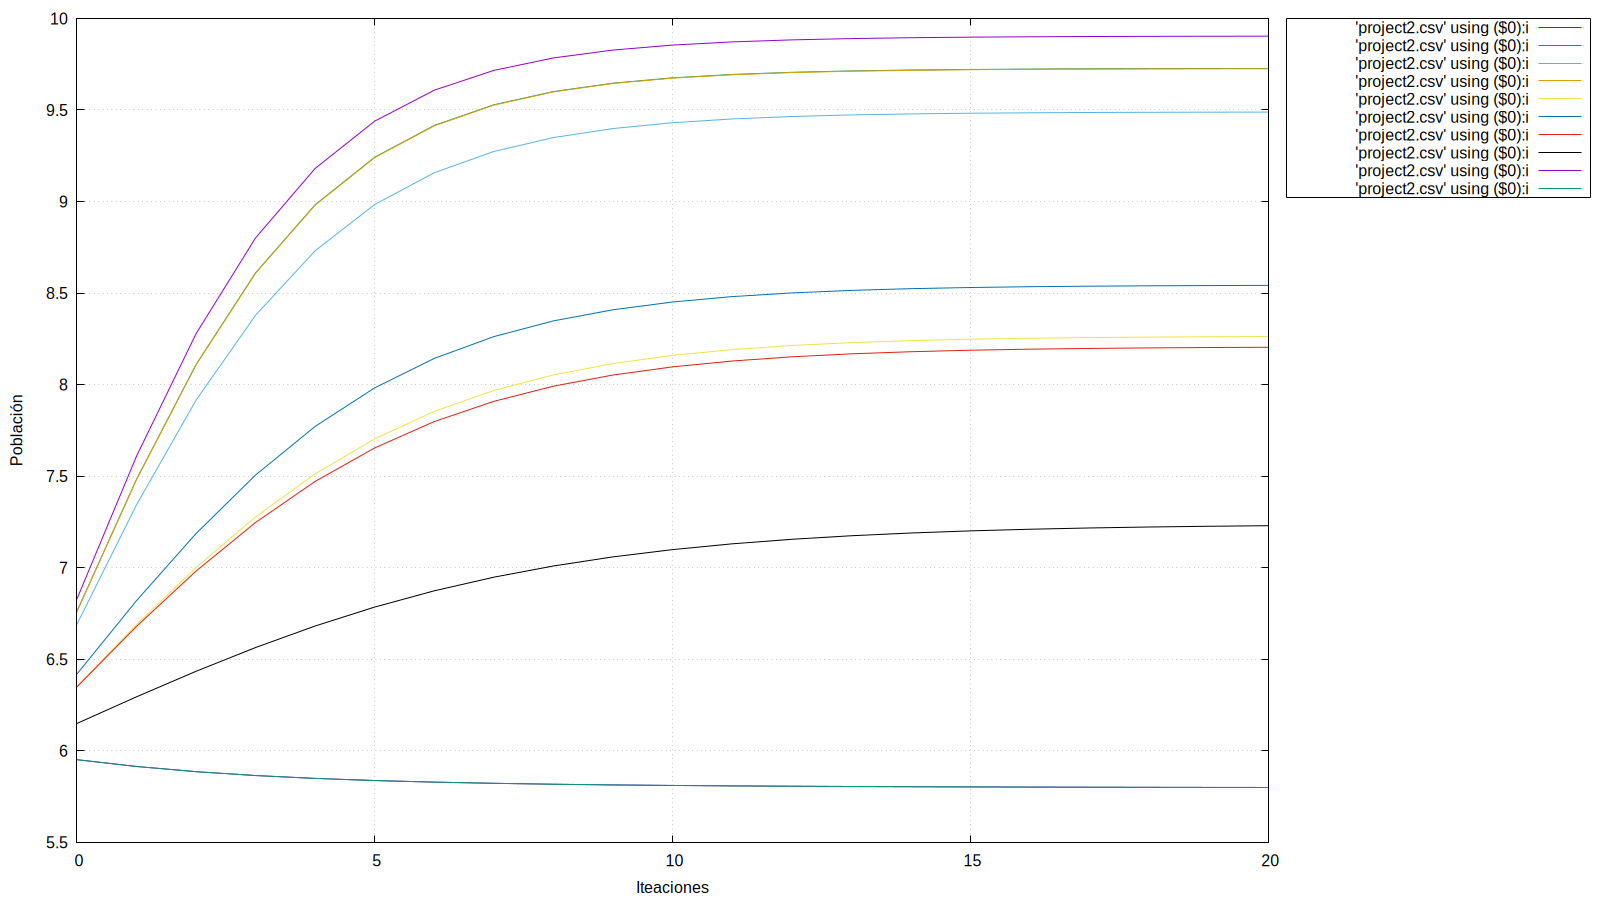
\includegraphics[width=10cm, height=10cm]{output_plot.png}
\caption{Aquí se puede observar la media del crecimiento de la población de las $x_{i}$ especies de plantas, al igual que en el anterior llega a un punto estable a partir de la iteración 600.}
\end{figure}

Una vez que se tiene el crecimiento de la población sin ninguna perturbación, a partir de esta simulación se desarrollan las diferentes perturbaciones.

\section{Eliminación de nodos}


La eliminación de nodos consiste en secuencialmente ir eliminando una fracción $f_{n}$ de nodos en $N$ pasos, para lo cual se selecciona un nodo no eliminado aún de la matriz $A_{ij}$ las interacciones de este nodo se vuelven 0 de manera que no aporte al sistema.
\begin{figure}[H]
     \label{fig-n-del}
     \includegraphics[width=10cm, height=10cm]{output_plot_x_fn_Two.png}
     \caption{Aquí se muestran 20 ejecuciones del programa con un $f_{n}=\frac{1}{10}$, en la parte de arriba de la gráfica se tienen los puntos obtenidos al ejecutar el programa con un estado inicial $x^{H}$ mientras que los puntos que caen a casi 0 son los correspondientes a $x^{L}$.}
     \end{figure}

\bibliographystyle{unsrt}
\bibliography{bibliografia} 
%\printbibliography 
\end{document}



